\documentclass[11pt]{amsart}
\usepackage{amsmath}
\usepackage{amssymb}
\usepackage{amsfonts}
\usepackage{enumitem}
\usepackage{amsthm}
\usepackage{mathrsfs}
\usepackage{csquotes}
\usepackage{listings}
\usepackage{color}
\usepackage[arrow,matrix,curve,cmtip,ps]{xy}
\usepackage{tikz}
\usetikzlibrary{shapes,shadows,arrows,trees,backgrounds}
\usepackage{graphicx}
\graphicspath{ {./Images/} }
\usepackage{thmtools}
\usepackage{hyperref}
\hypersetup{
    colorlinks=true,
    linkcolor=blue,
    filecolor=magenta,      
    urlcolor=cyan,
}

\allowdisplaybreaks
\theoremstyle{remark}
\newtheorem*{claim}{Claim}
\newtheorem*{exercise}{Exercise}
\newtheorem*{answer}{Answer}
\newtheorem*{question}{Question}
\newtheorem*{note}{Note}
\newtheorem*{sn}{Self Note} 
\newtheorem*{sd}{Self Definition} 
\newtheorem*{recall}{Recall} 

\newtheorem{theorem}{Theorem}[section]
\newtheorem{lemma}[theorem]{Lemma}
\newtheorem{proposition}[theorem]{Proposition}
\newtheorem{corollary}[theorem]{Corollary}
\newtheorem{notation}[theorem]{Notation}
\newtheorem*{theorem*}{Theorem}
\theoremstyle{remark}
\newtheorem{remark}[theorem]{Remark}
\newtheorem{definition}[theorem]{Definition}
\newtheorem{example}[theorem]{Example}
\newtheorem*{example*}{Example}
\newtheorem*{corollary*}{Corollary}
\newtheorem*{lemma*}{Lemma}
\newtheorem*{proposition*}{Proposition}


%this has equations numbered within sections 1.1,1.2, ... 2.1,...
\numberwithin{equation}{section}

%-------------------------------------------
%       Begin Local Macros
%-------------------------------------------
\newcommand{\Gal}{\mathrm{Gal}}
\newcommand{\Aut}{\mathrm{Aut}}
\newcommand{\Prob}{\mathbf{P}}
\newcommand{\Pow}{\mathcal{P}}
\newcommand{\F}{\mathcal{F}}
\newcommand{\M}{\mathcal{M}}
\newcommand{\A}{\mathcal{A}}
\newcommand{\B}{\mathcal{B}}
\newcommand{\E}{\mathcal{E}}
\newcommand{\n}{\noindent}
\newcommand{\Z}{\mathbb{Z}}
\newcommand{\N}{\mathbb{N}}
\newcommand{\Q}{\mathbb{Q}}
\newcommand{\R}{\mathbb{R}}
\newcommand{\C}{\mathbb{C}}
\newcommand{\T}{\mathbb{T}}
\newcommand{\im}{\operatorname{im}}
\newcommand{\coker}{\operatorname{coker}}
\newcommand{\ind}{\operatorname{ind}}
\newcommand{\rank}{\operatorname{rank}}
\newcommand\mc[1]{\marginpar{\sloppy\protect\footnotesize #1}}
%-------------------------------------------
%       end local macros
%-------------------------------------------

%-------------------------------------------
%      Begin Listing settings (Code)
%-------------------------------------------


\definecolor{codegreen}{rgb}{0,0.6,0}
\definecolor{codegray}{rgb}{0.5,0.5,0.5}
\definecolor{codepurple}{rgb}{0.58,0,0.82}
\definecolor{backcolour}{rgb}{0.95,0.95,0.92}
 
\lstdefinestyle{mystyle}{
    backgroundcolor=\color{backcolour},   
    commentstyle=\color{codegreen},
    keywordstyle=\color{magenta},
    numberstyle=\tiny\color{codegray},
    stringstyle=\color{codepurple},
    basicstyle=\footnotesize,
    breakatwhitespace=false,         
    breaklines=true,                 
    captionpos=b,                    
    keepspaces=true,                 
    numbers=left,                    
    numbersep=5pt,                  
    showspaces=false,                
    showstringspaces=false,
    showtabs=false,                  
    tabsize=2
}
 
\lstset{style=mystyle}

%-------------------------------------------
%      End Listing settings 
%-------------------------------------------




\begin{document}
\title{23 February 2017 Lecture: Learning Rules for Boltzmann Machines}
\author{Messina, Patrick\ 
	\and
	 Nabar, Aditi}

\date{\today}

\maketitle


%%%%%%%%%%%%%%%%%%%%%%%%%%%%%%%%%%%%%%%%%%%
\section{Database}
%%%%%%%%%%%%%%%%%%%%%%%%%%%%%%%%%%%%%%%%%%%

	This assignment had two objectives. The first was to build a generic
	Boltzmann machine and observe it's stabilization by monitoring the absolute 
	differences of the means from consecutive iterations. The second objective
	was to build a Restricted Boltzmann Machine $RBM$, train a set of weights
	for the reconstruction of some given input data, and using those weights to 
	initialize a multi-layer perceptron, perform a classification task. 

%%%%%%%%%%%%%%%%%%%%%%%%%%%%%%%%%%%%%%%%%%%
  \subsection{Define Features and Classes}
%%%%%%%%%%%%%%%%%%%%%%%%%%%%%%%%%%%%%%%%%%%
    Each image from the MNIST dataset is made of $28$ by $28$ or $784$
    pixels.  The set of features will be defined as $F = \{ F_1, F_2, \dots,
    F_{784} \}$ where each $F_p$ corresponds to a single pixel in a given image. 
    Each $F_p$ will store a value between $0$ and $1$ representing the amount 
    of gray intensity.  The higher or lower the number indicates the intensity of 
    dark or light color respectively.  The classes are defined by $C_1, C_2,\dots, 
    C_r, \dots, C_N$ where
    $N$ is the number of input data points, and the value assigned to
    each class $C_r$ is the label of image $r$. Though the classes are being 
    presented in this section, they are only relevant to the latter portion of the project.
    
    For the restricted Boltzmann machine, the RBM, the machine is non-deterministic. 
    It's goal is not to classify the input data into a set of classes. The job of the 
    restricted boltzman machine is to learn and reconstruct the input data, with high 
    probability. This obviously dictates the defining of the features as specified above.
    It also means that the size of the visible units $n_1$ will be the same as the 
    size of the reconstruction $n_3$, so that $n_1 = n_3$. 
	
%%%%%%%%%%%%%%%%%%%%%%%%%%%%%%%%%%%%%%%%%%%
  \subsection{Define Training and Test Sets}
%%%%%%%%%%%%%%%%%%%%%%%%%%%%%%%%%%%%%%%%%%%
    We are using the MNIST dataset which consists of 70,000 images of
    hand written numbers split into 60,000 points of training data,
    and 5,000 points of test data. 

%%%%%%%%%%%%%%%%%%%%%%%%%%%%%%%%%%%%%%%%%%%
\section{Software Tools}
%%%%%%%%%%%%%%%%%%%%%%%%%%%%%%%%%%%%%%%%%%%
	 The data set is loaded with the help of \textit{python-mnist}.
    \textit{Python-mnist} parses the MNIST dataset and returns two lists: the training set 
    and the test set. Both sets contained a list of images and list of labels. \textit{Scikit-learn}
    is used to analyze the performance of the model, namely with the help of the 
     \textit{pca} module. Finally, I used the module \textit{matplotlib} for 
     plotting the results of my analyses. 

    With computing the reconstruction and root mean-squared-error (RMSE) per batch,
    I was unable to run the batch-wise RMSE for the RBM on my local machine to 
    completion in a timely manner. Thus I am unable to show an assessment of the 
    RMSE across batches. 
  
%%%%%%%%%%%%%%%%%%%%%%%%%%%%%%%%%%%%%%%%%%%
\section{General Boltzmann Machines}
%%%%%%%%%%%%%%%%%%%%%%%%%%%%%%%%%%%%%%%%%%%
    A Boltzmann machine is a network of nodes that determine the state of the 
    nodes $x_i$ in a stochastic manner, where $x_i$ is defined as:
    \[ 
	x_i =     
    \begin{cases}
    {+1} & on\\
    {-1} & off
    	\end{cases}
    \]
    
    Upon presenting the machine with a binary vector
    representation of the data, the machine must then learn to reconstruct that 
    binary representation.  The machine accomplishes this by finding weights on
    certain connections so that the data vectors yield a low cost compared to 
    non-data binary vectors. The cost is measured in terms of the energy of the 
    configuration of the machine.
    
    The Boltzmann machine stochastic dynamics are as follows:
    - The Boltzmann machine iteratively and randomly steps through the set of 
    nodes. When the machine reaches each unit $i$, it computes a total value $v_i$ for
    each site. 
    \[
    	v = \sum_{i}{W_{ij}\cdot v_i}
    \]
    where $W_{ij} = W_{ji} \neq 0$. 
    
    The logistic sigmoid function will then use this value to compute a probability
    that after the visit to the node, the the node will take the On state. 
    \[
    	\Prob(y_i = +1) = \frac{1}{1 + e^{-v_i}}
    \]
    
    As long as the units continue to be updated in a stochastic manner, one in which
    the visitation is memory-less, then after a few full sweeps, the machine will achieve
    a stabilization of stochastic behavior that approximates a Boltzmann distribution 
    $G(x)$. In other words, $\Prob(X(t) = x) \simeq G(x)$. A Boltzmann distribution 
    determines the probability of a configuration based on the energy of that configuration,
    relative to other non-data binary vectors.
        \[
    	\Prob(y) = \frac{e^{-E(v)}}{\sum_u  e^{-E(u)}}
    \]
    
    Regardless of whether or not the machine approximates a Boltzmann 
    distribution, the energy of a configuration is given by
    
    \[
    	E(y) = \sum_i {x_i ^\text{y} \cdot b_i} - \sum_{i<j}{x_i ^\text{y} \cdot x_j ^\text{y} \cdot w_{ij}}
    \].    
	
	The Boltzmann machine was run with two sets of initial weights. The first set of 
	initial weights $W_1$ were randomly sampled from the interval $[-1, 1]$, and 
	the second set of weights was set to $W_2 = W_1 /10$.  Define stabilization 
	as the time (or sweep) $s(j)$ such that the absolute value of the difference of
	consecutive empirical means of unit $j$, or $|M_{s+t+1}(j) - M_{s+t}(j)|$, 
	remains below a set threshold for 10 consecutive sweeps. Given a threshold of 
	$0.01$, the general Boltzmann machine built for this project was observed to 
	stabilize at sweep 171 for $W_1$ and at sweep 271 for $W_2$.  The histograms 
	below demonstrate the differences in the quantiles of energy for the two weights. 
	The energy histogram for $W_1$ is right-skewed, while the energy histogram 
	for $W_2$ appears to be normally distributed with insignificant skew.
	
	\graphicspath{ {../Images/genericBM/} }
\begin{center}
 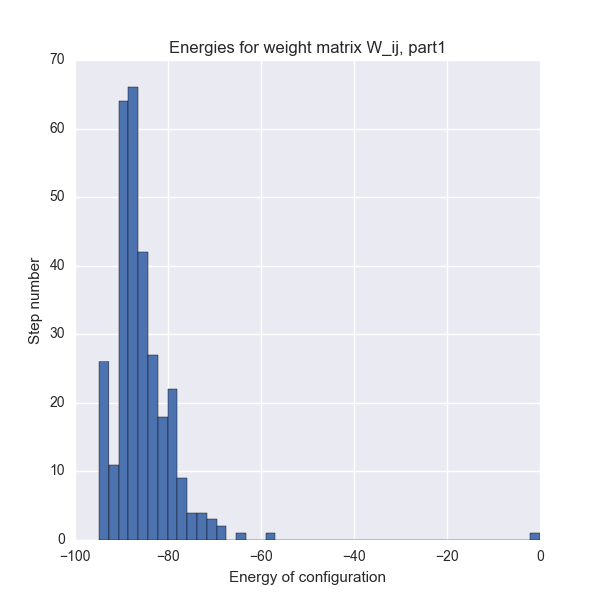
\includegraphics[width=.5\textwidth]{energies1.png}\hfill
  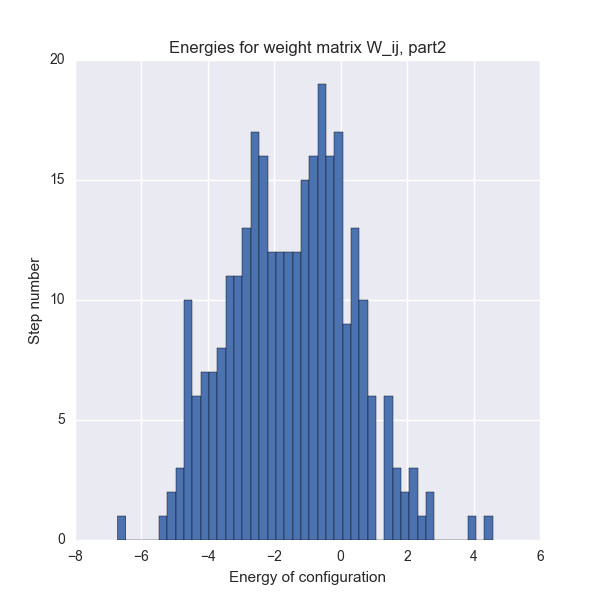
\includegraphics[width=.5\textwidth]{energies2.png}
\end{center}


%%%%%%%%%%%%%%%%%%%%%%%%%%%%%%%%%%%%%%%%%%%
\section{Fast RBMs}
%%%%%%%%%%%%%%%%%%%%%%%%%%%%%%%%%%%%%%%%%%%


	The algorithm used for the fast restricted Boltzmann machine is as follows. 
	The input data is broken into batches, which are fed into the machine as 
	visible units $visible_1$. These visible units are then passed into the logistic 
	sigmoid function along with their weights and biases, producing the hidden 
	units $hidden_1$. This computes the probabilities $\Prob(y_i = +1)$ for 
	the hidden nodes. Then $hidden_1$ is used to compute the probabilities for 
	reconstruction, or $visible_2$. $visible_2$ is then used to compute the
	probabilities for the hidden nodes $hidden_2$. $hidden_2$ is eventually 
	used for the contrastive divergence method used to update the weights, 
	but $visible_2$ is the desired reconstruction, after epochs 
	of training.
	
	The RMSE(W*) for the entire training data was found to be 1.10455, and the 
	corresponding observed RMSE for the whole test data was 0.81764. I am quite surprised that the 
	
	Due to lack of time and computational power, I was unable to compute the RMSE
	per batch. 
	
	
\subsubsection{Options for Initializing Weights}

	The following are options presented by \textit{Keras} for initializing the weights used 
	by a neural network.
	For the purposes of this project, the weight options were not that significant, as we were
	tasked with initializing the first layer of the multi-layer perceptron with weights trained 
	by the restricted	Boltzmann machine. The second layer however was initialized by 
	sampling from the normal distribution.
	
    Keras allows for the initialization of weights at the time the neural network 
    is initialized. Options for initialization include:
	\begin{itemize}
   	\item \textit{uniform}: sampling from the Uniform distribution	
    \textit{\item lecun\textunderscore uniform}: the Uniform multiplied by the 
    square root of the number of inputs as per Lecun 1998
    \textit{\item normal}: sampling from the Normal distribution
    \textit{\item identity}: generating as an identity matrix
    \textit{\item orthogonal}: generating as a random orthogonal matrix
    \textit{\item zeros}: generating a matrix of 0's
    \textit{\item ones}: generating a matrix of 1's 
    \textit{\item Glorot} initializations: Initialization using the Glorot method scaled by 
    $ fan_{in} + fan_{out}$.  With $W$ as the sampling distribution, $fan_{in}$ 
    as the number of inputs a hidden unit($a$) receives, and $fan_{out}$ as the 
    number of units the output of unit $a$ is sent to, Glorot's initialization samples 
    from the Normal (\textit{glorot\textunderscore normal}) or Uniform distributions
    (\textit{glorot\textunderscore uniform}), with $\mu = 0$ and $ \sigma $ given by 
    \[
    	\text{Var}(W) = \frac{2}{fan_{in} + fan_{out}}
    \]
    
    \textit{\item He} initializations: Initialization using the He method scaled by 
    $ fan_{in} $. With $W$ as the sampling distribution and $fan_{in}$ as the number 
    of inputs a hidden unit ($a$) receives, the He initialization methods, like the Glorot,
    sample from the Normal (\textit{he\textunderscore normal}) and the Uniform 
    (\textit{he\textunderscore uniform}) distributions with $\mu = 0$ and 
    $ \sigma $ given by
     \[
    	\text{Var}(W) = \frac{2}{fan_{in}}
    \]   
    
	\end{itemize}
	


\subsubsection{Options for Batch Learning}

    Using \textit{keras} makes it very easy to train a neural network. The \textit{model.fit}
    function is called using a \textit{batch\textunderscore size} parameter. When the parameter
    is given a value, the model is trained in batches. In the absence of the parameter,
    the model is processed as one large batch.
    
\subsubsection{Options for Stopping Learning}

	\textit{Keras} has an \textit{EarlyStopping} function in its \textit{Callbacks()} 
	class that will stop training when a specified quantity has stopped changing.
	This function allows for the monitoring of the following
	\begin{itemize}
	\item accuracy
	\item loss
	\item loss if validation is enabled during training 
	\item accuracy if the validation is enabled during training
	\end{itemize}
	allowing you to stop with specified conditions. \textit{Keras} allows
	for customizable parameters for monitoring. This is done by making a new class
	and inheriting from \textit{keras.callbacks.Callbacks()} and writing custom 
	values. The values can be gathered at the beginning of each batch, the end of
	a batch, or the end of an epoch. 

%%%%%%%%%%%%%%%%%%%%%%%%%%%%%%%%%%%%%%%%%%%%%%%%%%%%%%%%%%%%%%%%%%%%%%%%%%%%
  \subsubsection{Software Output}
%%%%%%%%%%%%%%%%%%%%%%%%%%%%%%%%%%%%%%%%%%%%%%%%%%%%%%%%%%%%%%%%%%%%%%%%%%%%
  We are able print the following performance measures: accuracy and loss. These measures can be printed
  per batch and per epoch. Any other output is done after training.


%%%%%%%%%%%%%%%%%%%%%%%%%%%%%%%%%%%%%%%%%%%
\section{PCA Analysis}
%%%%%%%%%%%%%%%%%%%%%%%%%%%%%%%%%%%%%%%%%%%
I conducted a principal component analysis (PCA) on the RBM on each hidden layer, 
given the training set and the test set. A principal component analysis isolates the 
$n$ components, or in this case, the $n$ learned features, that explain the variance
in the data. For this PCA, I set $n=3$ principal components. The number of components
needed to achieve 90\% of the energy in the model were observed as follows: \n
 
\begin{center}
  \small
  \tabcolsep=0.11cm 
 \begin{tabular}{ |c|c|c|c| } 
       \hline
		Data & Hidden Units & Number of Components \\
		\hline
		training & 32 & 23 \\
		test & 32 & 22 \\
		training & 64 & $>$32 \\
		test & 64 & $>$32 \\
       \hline
 \end{tabular}
 \end{center}


%%%%%%%%%%%%%%%%%%%%%%%%%%%%%%%%%%%%%%%%%%%
\section{Autoencoder Efficiency}
%%%%%%%%%%%%%%%%%%%%%%%%%%%%%%%%%%%%%%%%%%%

Using the weights trained for reconstruction by the restricted Boltzmann machine, I ran a 
multi-layer perceptron to classify the images, and to assess the performance of the RBM. 
After running 30 epochs, the MLP achieved a final loss of 0.2290, from an initial loss of 
0.3232. The accuracy of the MLP did not change significantly, increasing slightly from 
0.9000 to 0.9076. Since validation was enabled during training, the loss given 
validation and accuracy given validation are also relevant, and were observed to 
stop at 0.2266 and 0.9081 respectively. 

\graphicspath{ {../Images/restrictedBM/} }
\begin{center}
 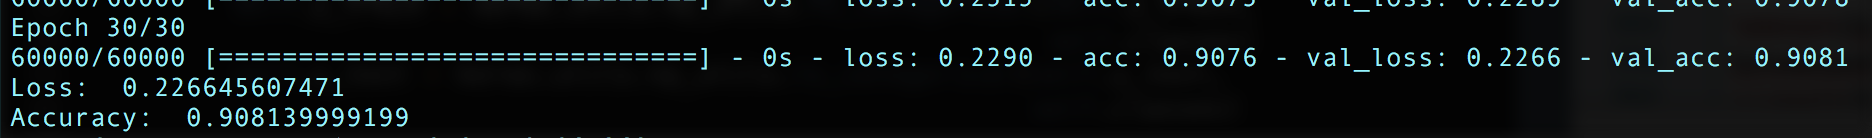
\includegraphics[width=1.25\textwidth]{scores.png}\hfill
\end{center}

\begin{thebibliography}{99}

\bibitem{keras}
Chollet, Fran\c{c}ois: Keras,
\\\texttt{https://github.com/fchollet/keras} 

\bibitem{NeuPy.com}
NeuPy.com
\\\texttt{https://neupy.com/2015/09/20/discrete\textunderscore hopfield\textunderscore network.html}

\bibitem{Scholarpedia.org}
Scholarpedia.org
\\\texttt{http://www.scholarpedia.org/article/Boltzmann\textunderscore machine\# The\textunderscore stochastic\textunderscore dynamics\textunderscore of\textunderscore a\textunderscore Boltzmann\textunderscore machine}

\bibitem{DeepLearning.net}
DeepLearning.net
\\\texttt{http://deeplearning.net/tutorial/rbm.html}

\end{thebibliography}
\end{document}
